% default values
\def\omegagh{10^2}  % omega_gh = omega_gu (Grenzfrequenz Hochpass bzw. untere Grenzfrequenz)
\def\omegagt{10^4}  % omega_gt = omega_go (Grenzfrequenz Tiefpass bzw. obere Grenzfreuquenz)

% Plot Umgebung:
\def\samples{41}

\def\xomegaordermin{0}
\def\xomegaordermax{6}
\def\xomegamin{1e\xomegaordermin}
\def\xomegamax{1e\xomegaordermax}

\def\yAmin{\xomegamin/\omegagh*0.8} % 0.8 für Platz für Steigungsdreiecke
\def\yAmax{1*2^0.5} % 2^0.5 für Platz

% Bandpass (Tiefpass 1. Ord + Hochpass 1. Ord) - Amplitudengang
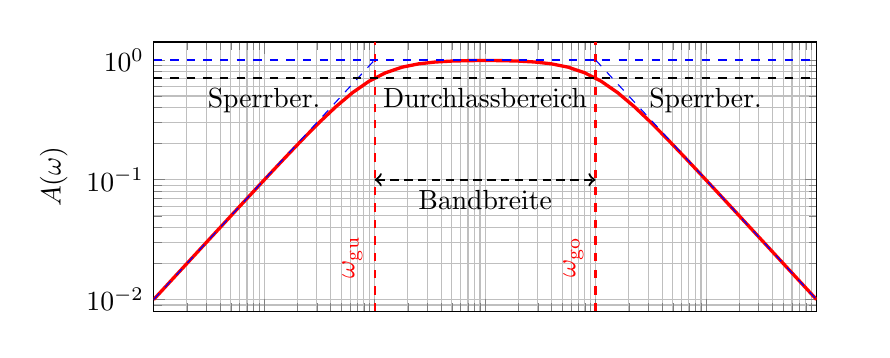
\begin{tikzpicture}[x=1mm,y=1mm] % gilt für tikz-coordinaten außerhalb der axis-environment
    \draw[draw=none] (-16,-2) rectangle (90,36); % Bildrahmen, Koordinatenbezug auf (0,0) des \begin{axis}...\end{axis} pgfplots, für
    \begin{loglogaxis}[
        %title={Bandpass},
        %xlabel={$\omega\ [\mathrm{Hz}]$},
        ylabel={$A(\omega)$},
        xmin=\xomegamin, xmax=\xomegamax,
        ymin=\yAmin, 
        ymax=\yAmax,   % \ymin needed as macro to draw ycomb with node-text from x-axis to plot intersection
        domain=\xomegamin:\xomegamax,
        samples=\samples,
        grid=minor,
        width=10cm,
        height=5cm,
        xticklabels={}, % remove x-axis labels
    ]
        % Plot: A(omega) = A_h(omega) * A_t(omega)
        \addplot+[mark=none,very thick,red,]   {1/(1+((\omegagh)/x)^2)^0.5 * 1/(1+(x/(\omegagt))^2)^0.5};   % A(omega) = 1/(1+(omega_gh/omega)^2)^0.5 * 1/(1+(omega/omega_gt)^2)^0.5
        
        % Grenzfrequenzen und Asymptoten
        \addplot+[dashed,mark=none,thick,red,] coordinates {(\omegagh,\yAmin)(\omegagh,\yAmax)}  node [pos=0.2,sloped,style={yshift=8pt}] {$\omega_{\mathrm{gu}}$}; % Grenzfrequenz
        \addplot+[dashed,mark=none,thick,red,] coordinates {(\omegagt,\yAmin)(\omegagt,\yAmax)}  node [pos=0.2,sloped,style={yshift=8pt}] {$\omega_{\mathrm{go}}$}; % Grenzfrequenz             
        \addplot+[dashed,mark=none,thick,blue] coordinates { (\xomegamin,1) (\xomegamax,1) };   % ungedämpft
        \addplot+[dashed,mark=none,blue,domain=\xomegamin:\omegagh]   { 1/(\omegagh/x) };       % ideal
        \addplot+[dashed,mark=none,blue,domain=\omegagt:\xomegamax]   { 1/(x/\omegagt) };       % ideal

        % Bandbreite
        \addplot+[<->,mark=none,thick,black] coordinates {(\omegagh,0.1)(\omegagt,0.1)} node [pos=0.5,anchor=north] {Bandbreite}; % static y pos
        % Bereiche
        \addplot+[dashed,mark=none,black,]  coordinates { (\xomegamin, 1/2^0.5) ( \xomegamax, 1/2^0.5) }   
            %node [pos=0,anchor=west,clip=false,yshift=-12pt] {$\frac{1}{\sqrt{2}}$}  % clipped away, otherwise asymptote peaks out above
            node [pos=0.1666,anchor=north] {Sperrber.}       % static
            node [pos=0.5,anchor=north]  {Durchlassbereich}     % static
            node [pos=0.666+0.1666,anchor=north] {Sperrber.} % static
        ;
    \end{loglogaxis}
\end{tikzpicture}